\documentclass[12pt,openright,a4paper]{article}

\usepackage{hyperref}
\usepackage[T1]{fontenc}
\usepackage[utf8]{inputenc}
\usepackage[italian]{babel}
\usepackage{amsmath}
\usepackage{amssymb}
\usepackage{caption}
\usepackage{graphicx, floatflt}
\usepackage{booktabs}
\usepackage{textcomp}
\usepackage{subfig}

% permette di inserire le note a margine
\usepackage{marginnote}


\begin{document}
\title{Analisi di Matrici di Correlazione di Soggetti ADNI2 e ABIDE Tramite Network Growth}
\author{Carlo Mengucci}

\maketitle

\tableofcontents

\section{Introduzione}

\textit{Questo lavoro ha l'obiettivo di analizzare le matrici di correlazione di soggetti provenienti dai database ADNI (Alzheimer) e ABIDE (Autismo), tramite osservazione della dinamica di crescita dei Networks estratti dalle matrici stesse.}

\textit{E' analizzata la capacità di separazione dei soggetti di entrambi i database in relazione  all'andamento del numero dei nodi al crescere dei links, del numero di componenti connesse al crescere dei links, della dimensione della componente connessa maggiore al crescere dei links.}

\textit{Vengono inoltre presentate per il confronto diverse ipotesi di generazione random; in particolare sono state prese in considerazione una generazione tramite Teorema del cerchio di Gershgorin, una generazione tramite distribuzione di Wishart, con matrice di scala pari alla media delle matrici di correlazione dei soggetti AD per il database ADNI e dei soggetti CTRL per le matrici ABIDE, una generazione completamente random (Erdos-Renyi).}

\section{Struttura dei Databases}

\subsection{Database ADNI}

Dei 403 soggetti totali sono stati utilizzati 232 soggetti a seguito di operazioni di filtraggio e dell'individuazione di discrepanze nelle procedure di normalizzazione. 

E' infatti possibile riscontrare la presenza di due gruppi distinti all'interno del database, dei quali è stato preso in considerazione il più numeroso, formato da circa 300 soggetti.

Dei 300 soggetti, 232 sono stati utilizzati per l'elaborazione finale. Sono infatti stati esclusi dallo studio i soggetti appartenenti alla categoria \textit{MCI, Mild Cognitive Impairment}, in modo da considerare esclusivamente soggetti \textit{san}i \textit{NC} e \textit{malati} \textit{AD}.

 La presenza di soggetti per il gruppo \textit{AD} è del $63 \% $ mentre il restante  $37 \%$ dei 232 soggetti considerati appartiene al gruppo \textit{NC}.

Ad ogni soggetto è associata una matrice di correlazione $N\times N$, $N=549$, Ognuno degli N elementi rappresenta un \textit{Macrovoxel} di cui è estratta la correlazione \textit{topologica} rispetto a tutte le altre componenti del sistema. Ogni \textit{Macrovoxel} è definito su un insieme di $3\cdot10^3$ Voxel.

\subsection{Database ABIDE}

Dei soggetti ABIDE è stato utilizzato soltanto il cluster proveniente dalla New York University, di cui sono stati isolati i soggetti di sesso maschile.

La classificazione è esclusivamente binaria \textit{(CTRL=controlli, AUT=autistici)}, l'analisi non tiene pertanto conto dei diversi gruppi diagnostici.

In totale sono stati dunque analizzati 136 soggetti ABIDE, con una percentuale di controlli pari al $53\%$ dei soggetti totali; il restante $47\%$ dei soggetti è dunque rappresentativo del gruppo degli autistici.

 Ad ogni soggetto è associata una matrice di correlazione $N\times N$, $N=116$, Ognuno degli N elementi rappresenta un \textit{Macrovoxel} di cui è estratta la correlazione \textit{funzionale} rispetto a tutte le altre componenti del sistema.

\section{Network Growth}

Per lo studio della dinamica di crescita dei networks è stato eseguito un ranking sul valore assoluto degli elementi delle matrici di correlazione. In questo modo è possibile ottenere un network per ogni paziente, a partire dai link associati ai più alti valori di correlazione fra le componenti del sistema. 

Nel caso presente, sia per ADNI che per ABIDE, le componenti del sistema sono costituite dai macrovoxel in cui l'immagine fMR associata ad ogni paziente è stata inizialmente suddivisa.

Viene dunque osservata la crescita del network in relazione al numero di link aggiunti in maniera sequenziale, in termini di \textit{numero totale dei nodi}, \textit{numero di componenti connesse}, \textit{dimensione della componente connessa maggiore}.

Un esempio di Network ottenuto attraverso questa procedura è riportato in fig.\ref{ADNI50}.

\begin{figure}[!h]
\centering
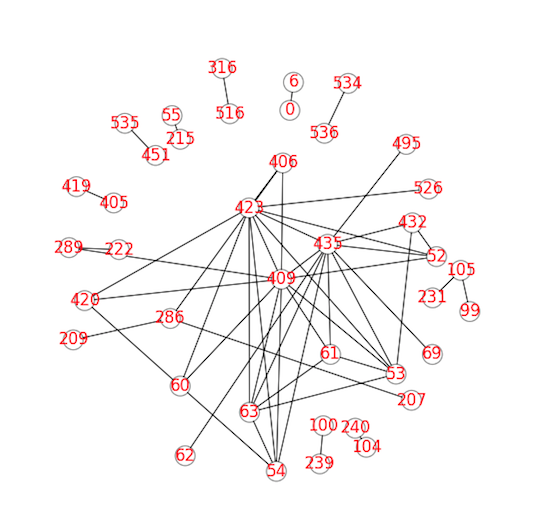
\includegraphics[scale=0.4]{ADNI50c}
\caption{\textit{Esempio di Network ottenuto da un paziente ADNI di classe AD. Il network è costruito a partire dai primi 50 link forniti dal sorting.}}
\label{ADNI50}
\end{figure}

\section{Random Models and Generators}

In questa sezione sono presentate le metodologie di generazione per le ipotesi random di confronto.

Essendo per natura le matrici di correlazione \textit{simmetriche definite positive}, la scelta per i modelli è ricaduta su due metodi principali: \textit{il teorema del cerchio di Gershgorin}, che permette di generare matrici simmetriche definite positive a partire dalla generazione semi-random dei propri elementi e un sampling ottenuto da una \textit{distribuzione di Wishart}. 

Quest'ultima permette l'estrazione di un campione random di matrici simmetriche definite positive a partire da una\textit{ matrice di scala} nota e dalla definizione dei gradi di libertà del sistema.

\subsection{Generazione di Gershgorin}

Un metodo rapido per generare matrici random simmetriche definite positive è quello di sfruttare il \textit{Teorema del Cerchio di Gershgorin}.
Esso è costituito dalla seguente affermazione:

\textit{sia $A$ una matrice complessa $n \times n$ con elementi $a_{ij}$; per $i\in[1...n]$ sia $R_i=\sum_{j \neq i}\mid a_{ij} \mid$ la somma dei valori assoluti   degli elementi non diagonali della riga i-esima. Sia  $D(a_{ii}, R_i)$ il disco centrato in $a_{ii}$ di raggio $R_i$. Ogni autovalore di $A$ è contenuto all'interno di almeno uno dei dischi di Gershgorin $D(a_{ii}, R_i)$.} \cite{Gershgorin}

Generando dunque elementi non diagonali $ a_{ij}$ \textit{Random} tali che $ \mid a_{ij} \mid \leqslant \epsilon$ con $ \epsilon = \frac{1}{4} $ si ottiene che tutti gli autovalori della matrice risultante cadano all'interno di un \textit{cerchio di Gershgorin} di raggio 1 centrato in 1 \footnote{\textit{Nota: Tale risultato numerico è dimostrato in \cite{Gershgorin}}}. Poichè gli autovalori di una matrice simmetrica reale sono reali, tutti gli autovalori saranno positivi.

\subsection{Generazione Tramite Distribuzione di Wishart}

La distribuzione di Wishart consiste in una famiglia di distribuzioni per \textit{matrici simmetriche definite positive}.

\textit{Def.} Siano $X_1...X_n$ indipendenti $N_p(0,\Sigma)$ distribuiti, tali da formare una matrice di dati $p\times n$, $X=[X_1...X_n]$.
La distribuzione di \textit{matrici random} $p\times p$, $M=XX'=\Sigma^n_{i=1}X_iX_i'$ è una distribuzione di Wishart. \cite{AMS}

La matrice random $M_{p\times p}=\Sigma^n_{i=1}X_iX_i'$ segue una distribuzione di Wishart a $n$ gradi di libertà e \textit{matrice di covarianza} $\Sigma$ ed è definita $M\sim W_p(n, \Sigma)$.
Per $n\geq p$ la \textit{pdf} di $M$ assume la forma   \footnote{\textit{Nota: $\|\Sigma , N \| = det (\Sigma , M)$}}:  
\begin{equation}
f(M)=\frac{1}{2^{\frac{np}{2}}\Gamma_p(\frac{n}{2})\|\Sigma\|^{\frac{n}{2}}}\|M\|^{\frac{n-p-1}{2}}exp[-\frac{1}{2}trace(\Sigma^{-1}M)]
\label{Wishart-pdf}
\end{equation}

La Wishart può essere interpretata come l'estensione multivariata di una distribuzione $\chi^2$.

Utilizzando come matrice di scala la matrice media di categoria e conoscendo i gradi di libertà del sistema, è possibile generare un sampling di matrici di correlazione da utilizzare per generare networks tramite ranking.

\textit{Per il lavoro presente, sono state utilizzate funzioni e toolkit di Wishart Random Smapling del modulo Python 3.6 Scipy.Stats.}

\section{Risultati}

\subsection{Soggetti ADNI}

Prendendo in analisi la fig.\ref{ADNI-ADNC}, si evince che non è possibile separare le due categorie di soggetti presi in esame osservando la dinamica di crescita del network.

\begin{figure}[!h]
\centering
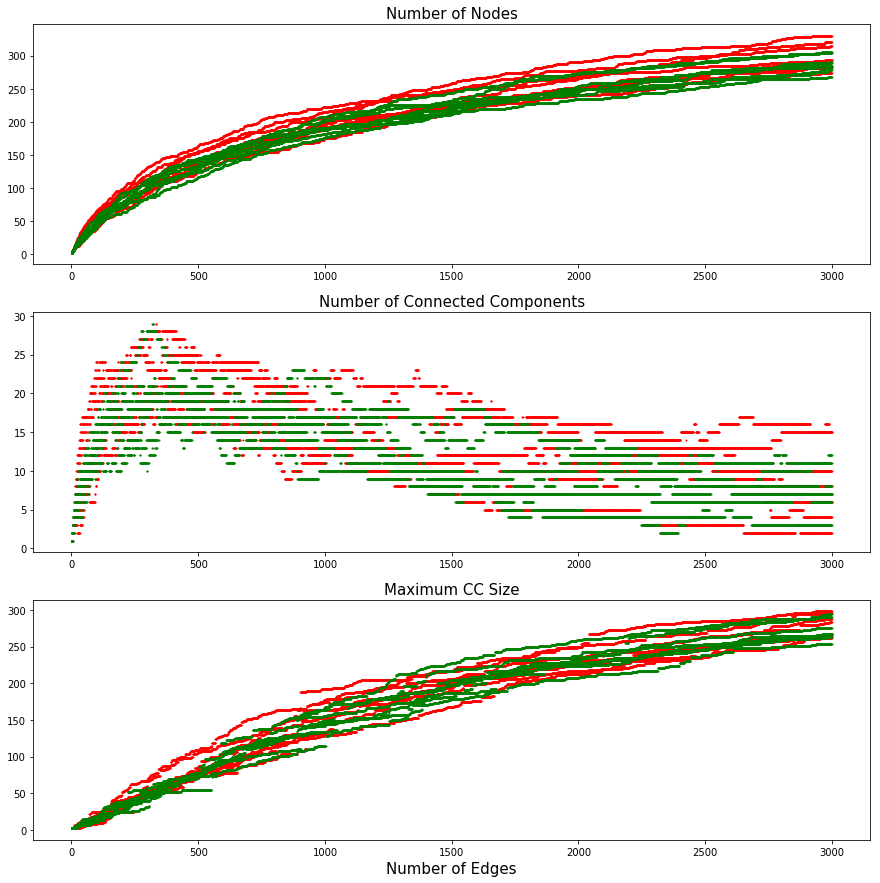
\includegraphics[scale=0.4]{Network-growth}
\caption{\textit{Crescita dei Network di 8 soggetti AD, in rosso, e 8 soggetti NC, in verde.}}
\label{ADNI-ADNC}
\end{figure}

Un risultato interessante si trova però confrontando le crescite dei soggetti con i modelli random proposti. 

Osservando la fig.\ref{ADNI-ALL} si vede come la crescita dei network dei soggetti ottenuti tramite \textit{Wishart Sampling} sia confrontabile con i pazienti reali, mentre la crescita dei network completamente random si distacca in termini di andamento. La distribuzione Wishart costituisce dunque una buona ipotesi nulla per le matrici ADNI.

\begin{figure}[!h]
\centering
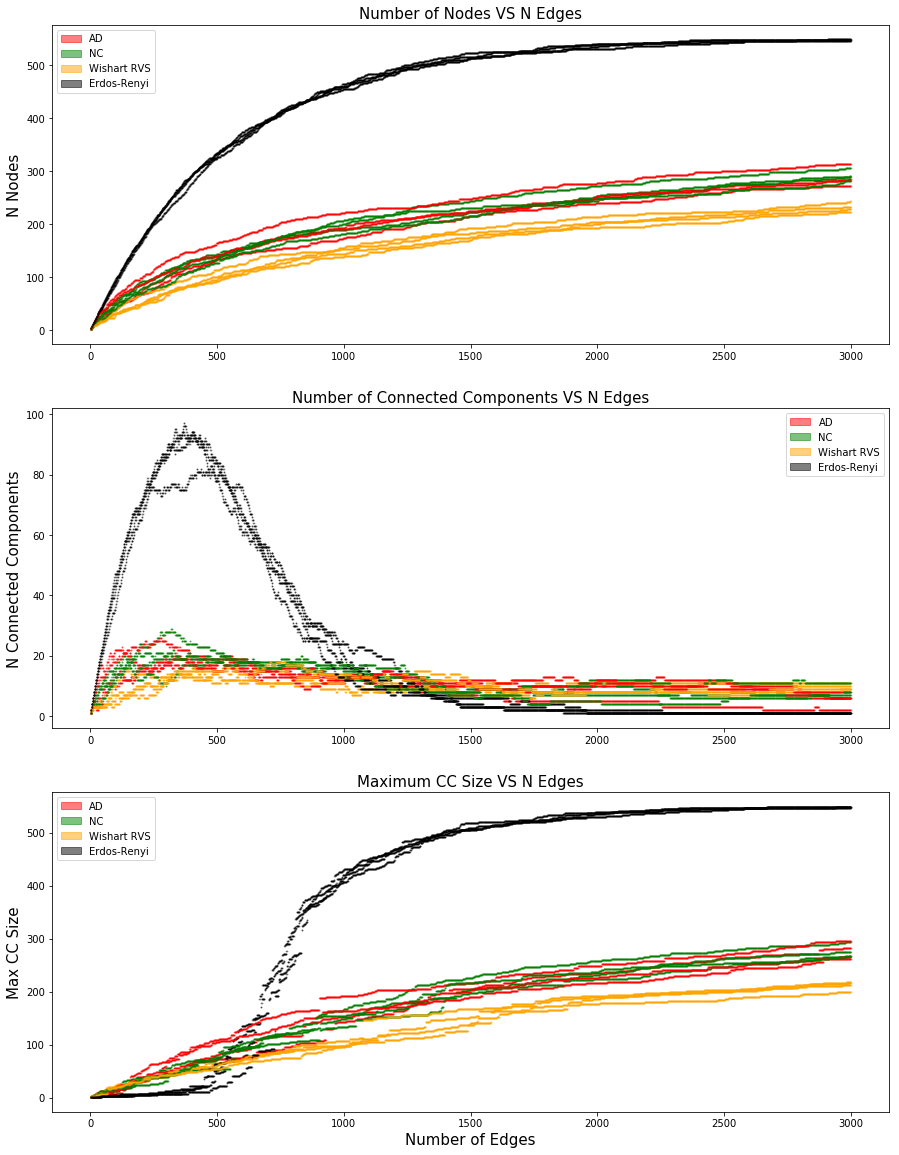
\includegraphics[scale=0.4]{ALL-Network-growthSMAD}
\caption{\textit{Crescita dei Network di 4 soggetti AD, 4 soggetti NC e 4 soggetti random sample. }}
\label{ADNI-ALL}
\end{figure}

Come analisi finale è stata elaborata una Lowess Regression sulle curve medie di 20 soggetti AD e 20 soggetti NC (fig.\ref{ADNI-Average}). Il range dei valori in x è stato discretizzato in 40 bins, la cui varianza è praticamente nulla dato l'alto numero di valori campionati per ogni soggetto.   Purtroppo il tool utilizzato per l'elaborazione non permette la visualizzazione dell'intervallo di confidenza per una regressione di tipo Lowess. Vi è ad ogni modo una discriminazione maggiore rispetto all'analisi per singoli soggetti riportata in fig.\ref{ADNI-ALL}.

\begin{figure}[!h]
\centering
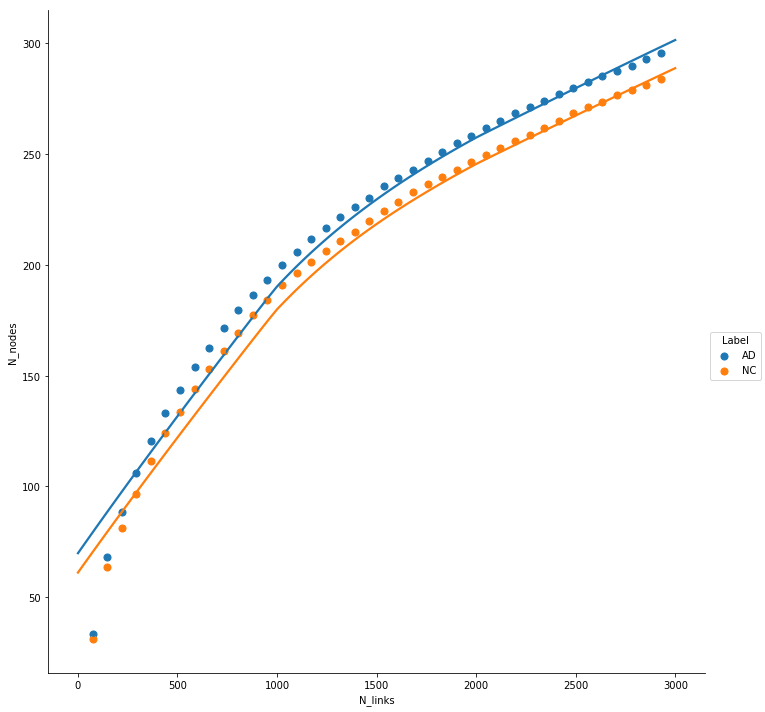
\includegraphics[scale=0.4]{Average-Lowess20}
\caption{\textit{Crescita media dei Network di 20 soggetti AD e 20 soggetti NC. Le linee rappresentano la regressione di Lowess. }}
\label{ADNI-Average}
\end{figure}

\clearpage

\subsection{Soggetti ABIDE}

Prendendo in analisi la fig.\ref{ABIDE-CTRLAUT}, si evince che non è possibile separare le due categorie di soggetti presi in esame osservando la dinamica di crescita del network.

\begin{figure}[!h]
\centering
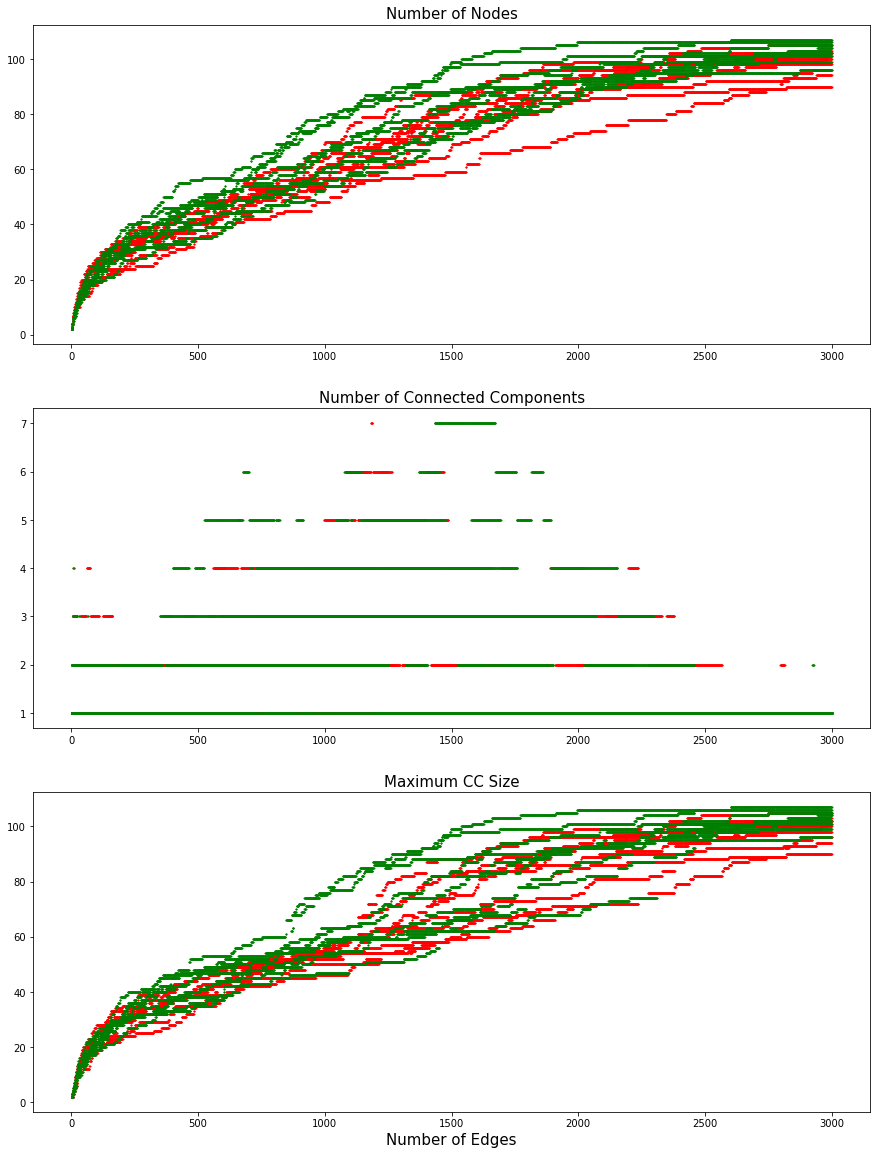
\includegraphics[scale=0.4]{ABIDE-Network-growth}
\caption{\textit{Crescita dei Network di 8 soggetti AUT, in rosso, e 8 soggetti CTRL, in verde.}}
\label{ABIDE-CTRLAUT}
\end{figure}

Confrontando anche in questo caso i soggetti con le ipotesi di generazione random, come mostrato in fig.\ref{ABIDE-ALL}, si nota come la generazione di Gershgorin converga con quella completamente random. Leggermente più affine all'andamento di soggetti è la crescita dei network ottenuti tramite \textit{Wishart Sampling}, anche se la similitudine è minore rispetto a quella ottenuta per le matrici ADNI. Un dettaglio degli andamenti delle ipotesi random è riportato in fig. \ref{ABIDE-RAND}.

\begin{figure}[!h]
\centering
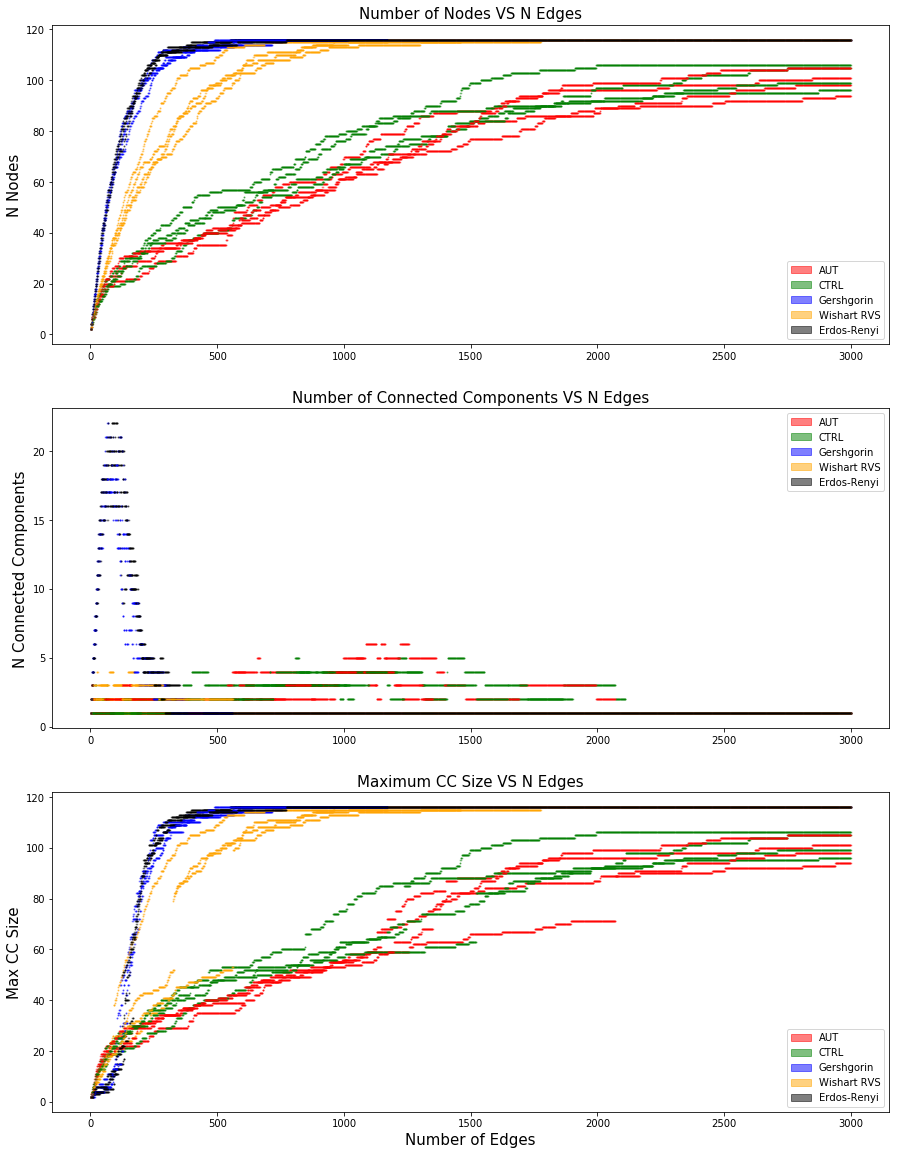
\includegraphics[scale=0.35]{ALL-Network-growthSMC}
\caption{\textit{Crescita dei Network di 4 soggetti AUT,  4 soggetti CTRL e 4 soggetti random sample}}
\label{ABIDE-ALL}
\end{figure}

\begin{figure}[!h]
\centering
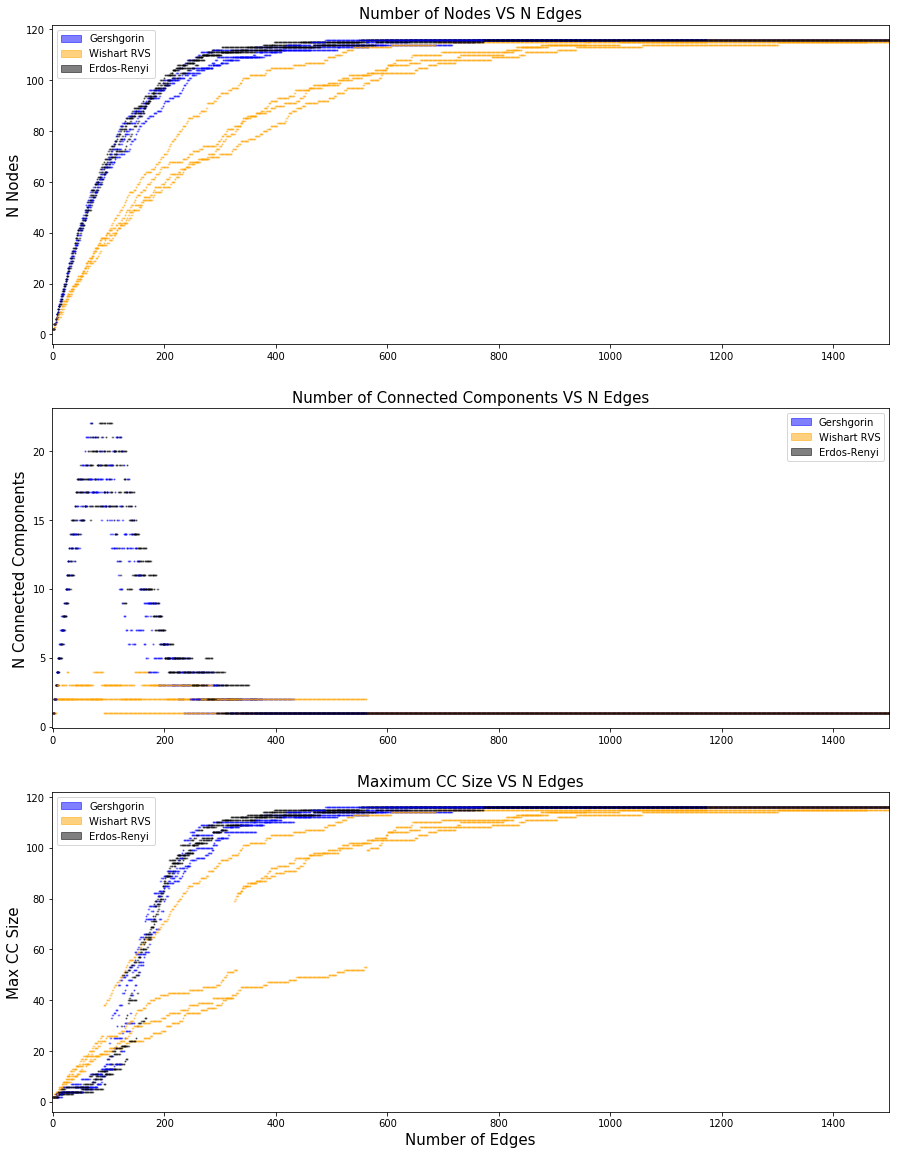
\includegraphics[scale=0.4]{ALL-RNetwork-growth}
\caption{\textit{Dettaglio del confronto tra ipotesi random per matrici ABIDE.}}
\label{ABIDE-RAND}
\end{figure}

Come analisi finale è stata elaborata una Lowess Regression sulle curve medie di 50 soggetti AUT e 50 soggetti CTRL (fig.\ref{ABIDE-Average}). Il range dei valori in x è stato discretizzato in 40 bins, la cui varianza è praticamente nulla dato l'alto numero di valori campionati per ogni soggetto.   Purtroppo il tool utilizzato per l'elaborazione non permette la visualizzazione dell'intervallo di confidenza per una regressione di tipo Lowess. Non è ad ogni modo possibile osservare una discriminazione, in accordo con quanto ottenuto e riportato in fig.\ref{ABIDE-ALL}.

\begin{figure}[!h]
\centering
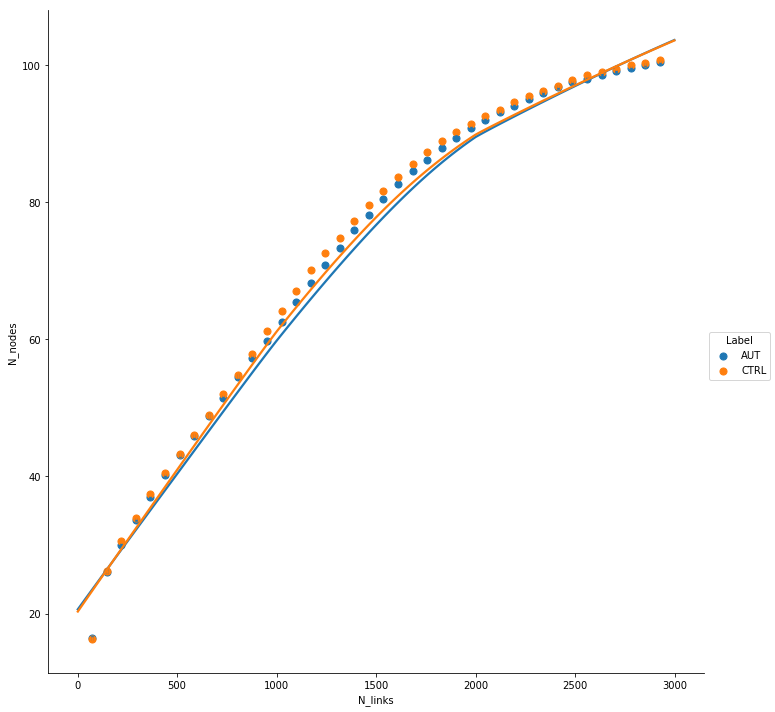
\includegraphics[scale=0.4]{ABIDE-Average-Lowess50}
\caption{\textit{Crescita media dei Network di 50 soggetti AUT e 50 soggetti CTRL. Le linee rappresentano la regressione di Lowess. }}
\label{ABIDE-Average}
\end{figure}

\clearpage

\begin{thebibliography}{99}

\bibitem{Gershgorin}
Golub, G. H.; Van Loan, C. F. 

\emph{Matrix Computations}

Baltimore: Johns Hopkins University Press, 1996

\bibitem {AMS}
Hardle, Wolfgang and Leopold Simar

\emph{Applied Multivariate Statistical Analysis}

Heidelberg: Springer Berlin Heidelberg, 2012


\end{thebibliography}

\end{document}


